\begin{homeworkProblem}

\textbf{Optional: Hugging Face Course in Deep RL.} Welcome to \href{https://huggingface.co/learn/deep-rl-course/unit0/introduction}{Hugging Face Course in Deep RL}! This is an educational resource produced by Hugging Face community that makes it easier to learn about deep reinforcement learning (deep RL).

(a) Finish basic units including unit 1(Introduction to Deep Reinforcement Learning), unit 2(Introduction to Q-Learning), unit 3(Deep Q-Learning with Atari Games), unit 4(Policy Gradient with Pytorch), unit 6(Actor-Critic Methods with Robotics Environments), unit 8(Proximal Policy Optimization)

(b) (Bonus)Finish all remaining units

\solution

The finished units: 1, 2, 3, 4, 6, 8's codes cuold be check in `code/Huggingface\_Deep\_RL'.

Aftering running the implemented codes, several models from different units were pushed to to the Huggingface Hub, and the models are as follows:
\begin{figure}[h]
    \centering
    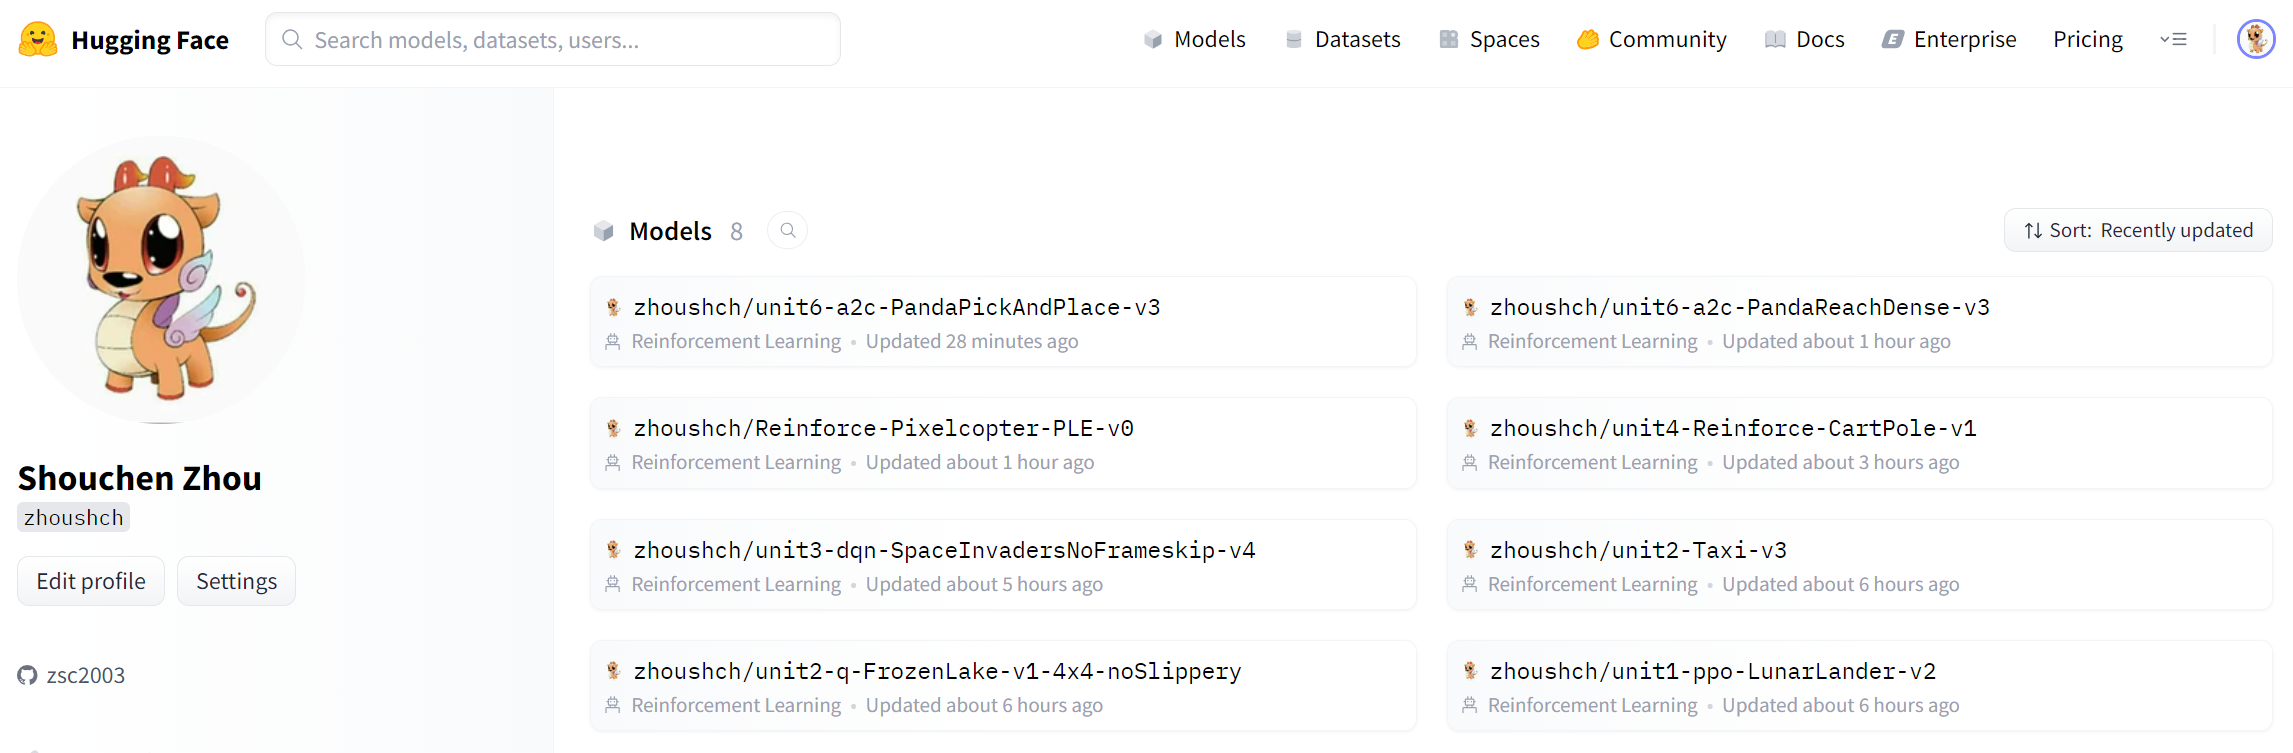
\includegraphics[width=0.8\textwidth]{../Img/Huggingface_DRL/models.png}
\end{figure}

The quizzes of each units are also finished, which could be seen as follows:
\begin{figure}[H]
    \centering
    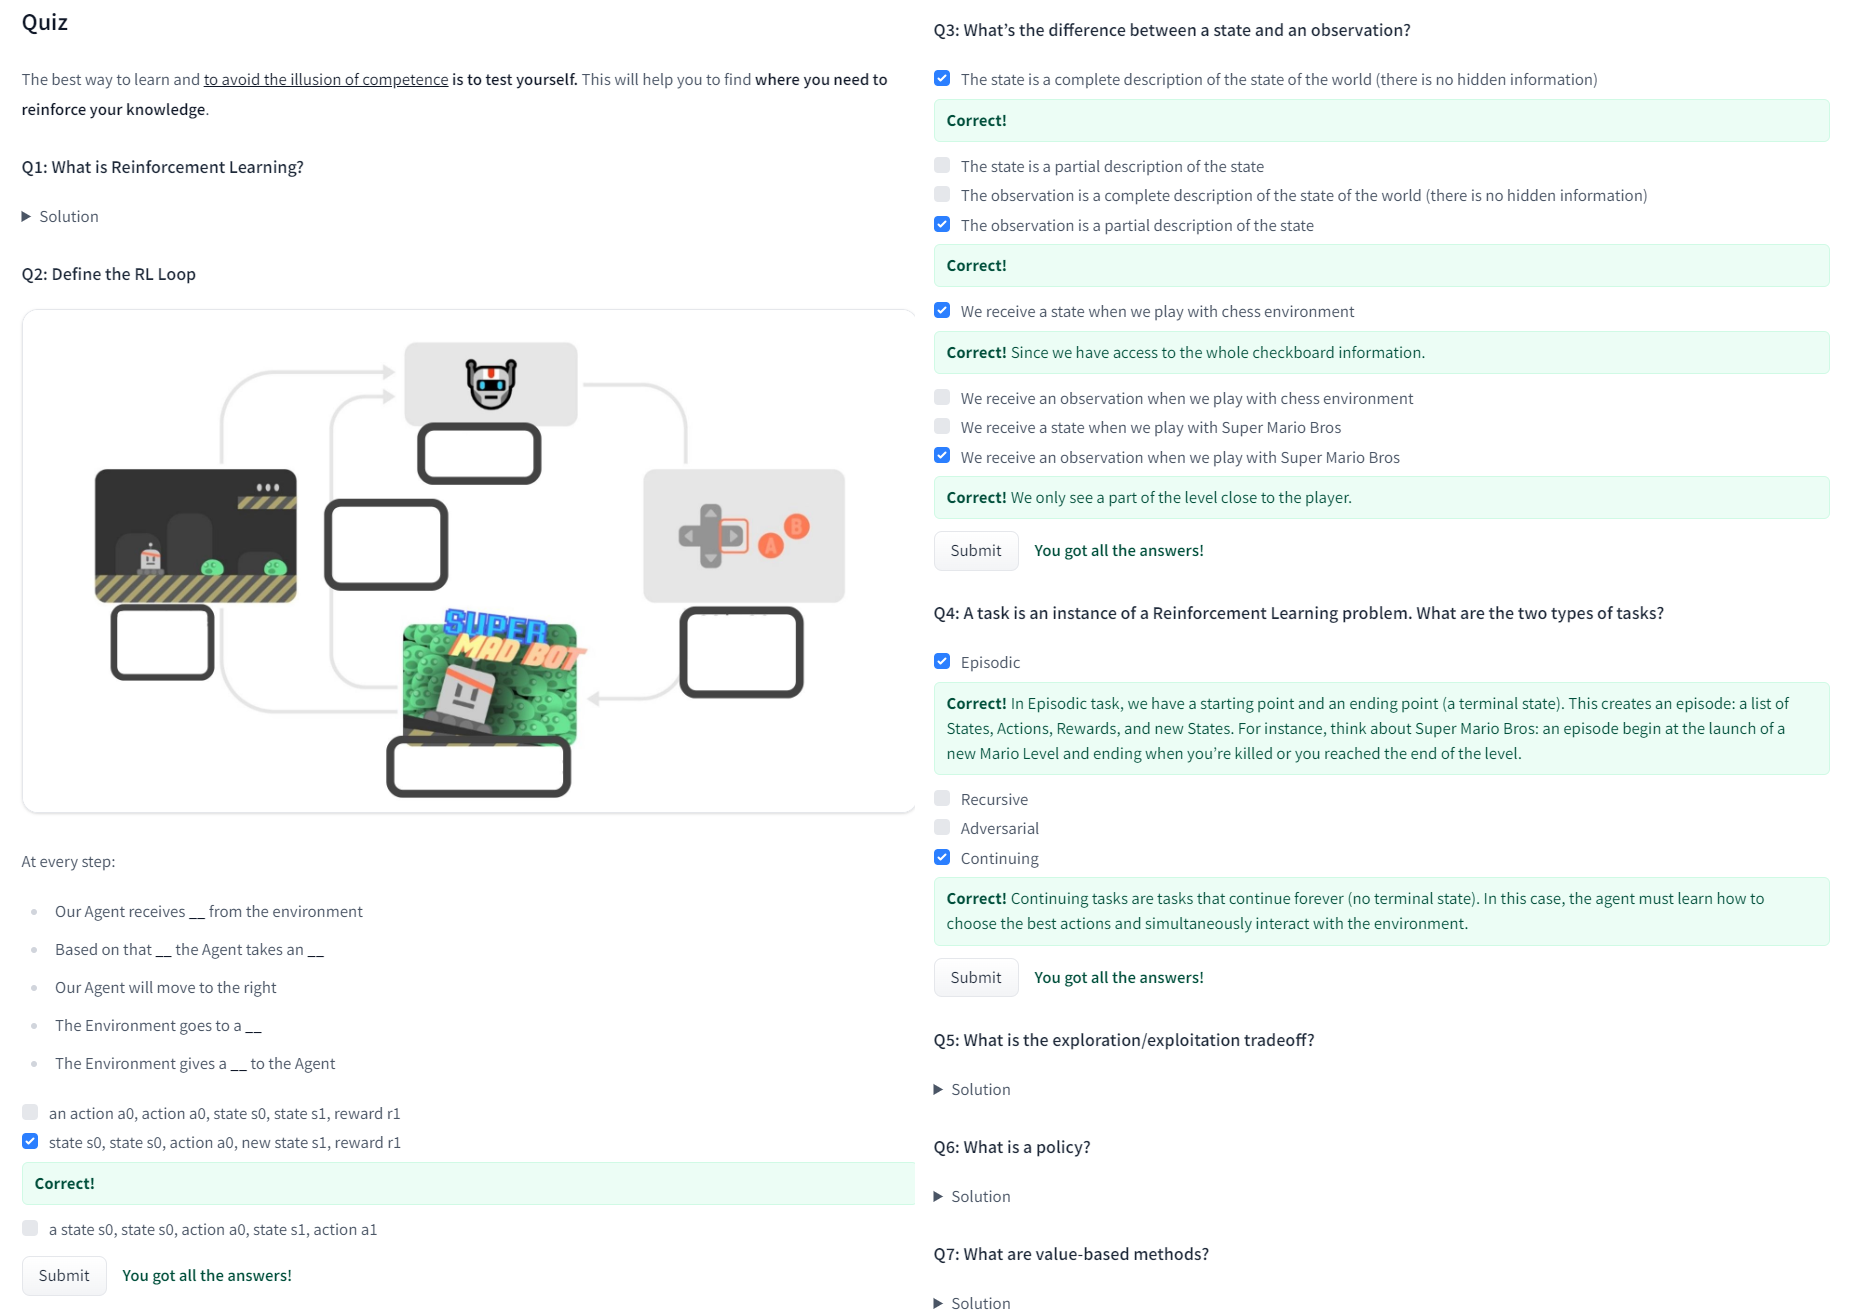
\includegraphics[width=0.8\textwidth]{../Img/Huggingface_DRL/unit1_quiz.png}
\end{figure}
\begin{figure}[H]
    \centering
    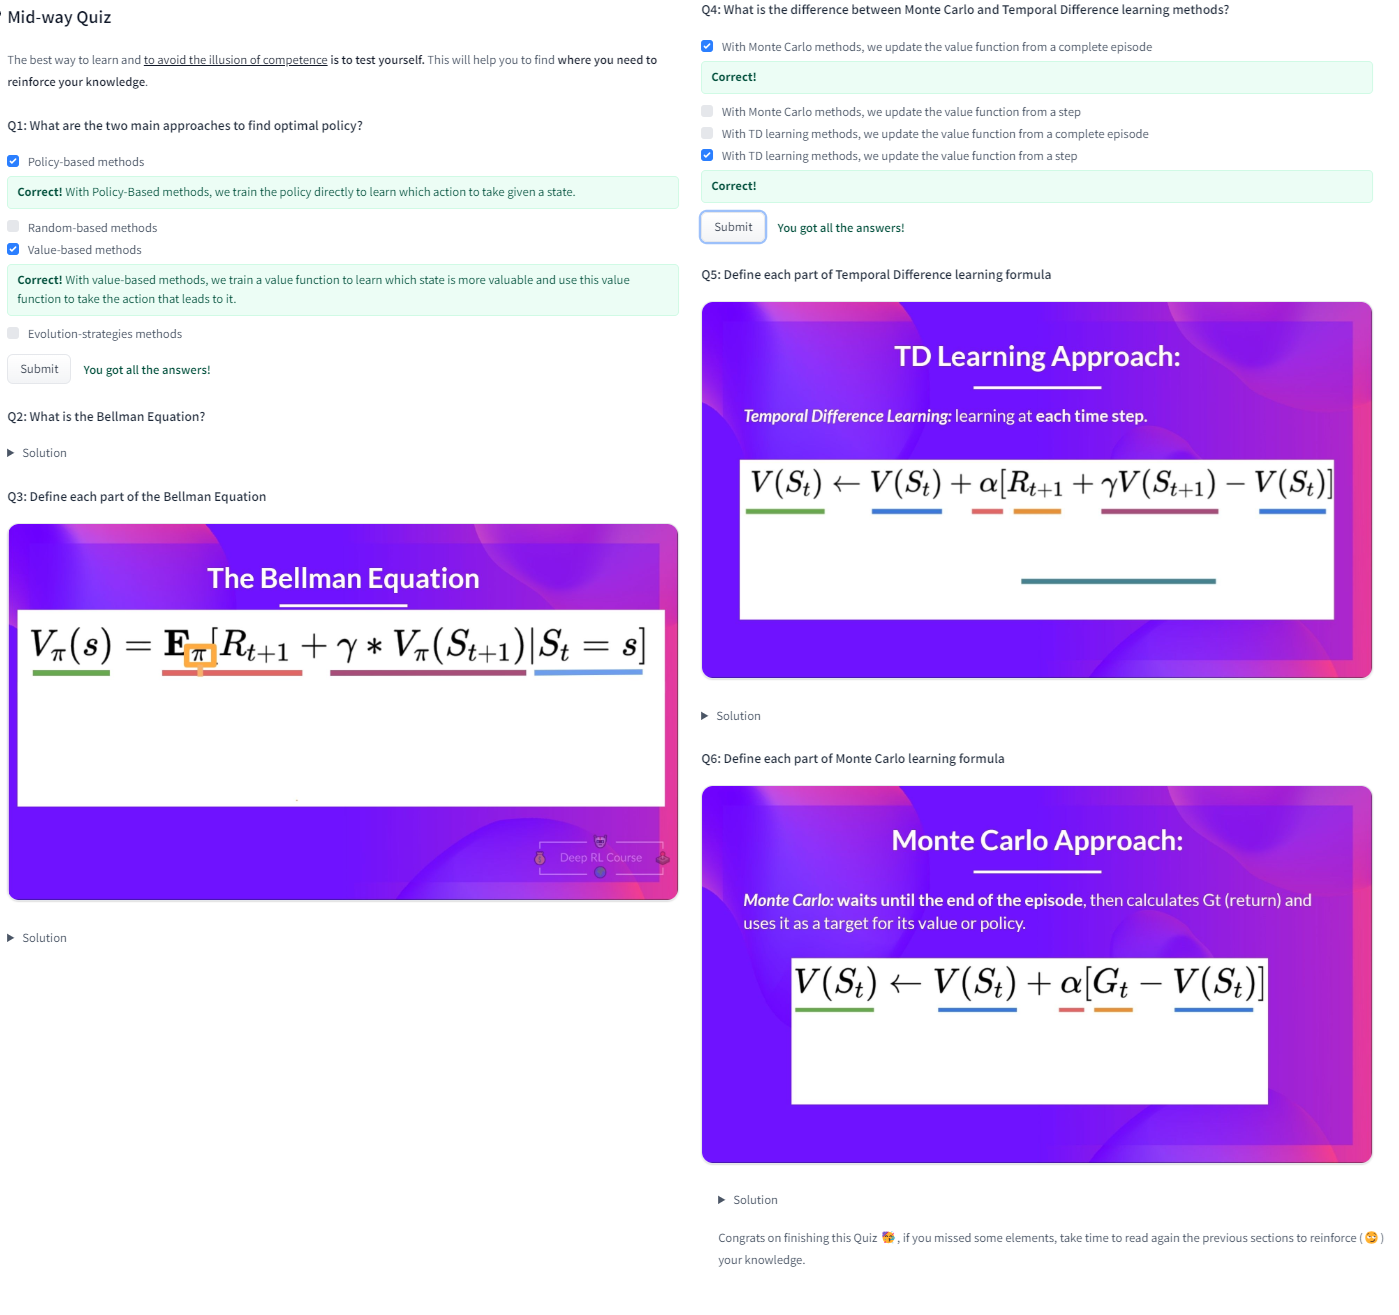
\includegraphics[width=0.8\textwidth]{../Img/Huggingface_DRL/unit2_midway_quiz.png}
\end{figure}
\begin{figure}[H]
    \centering
    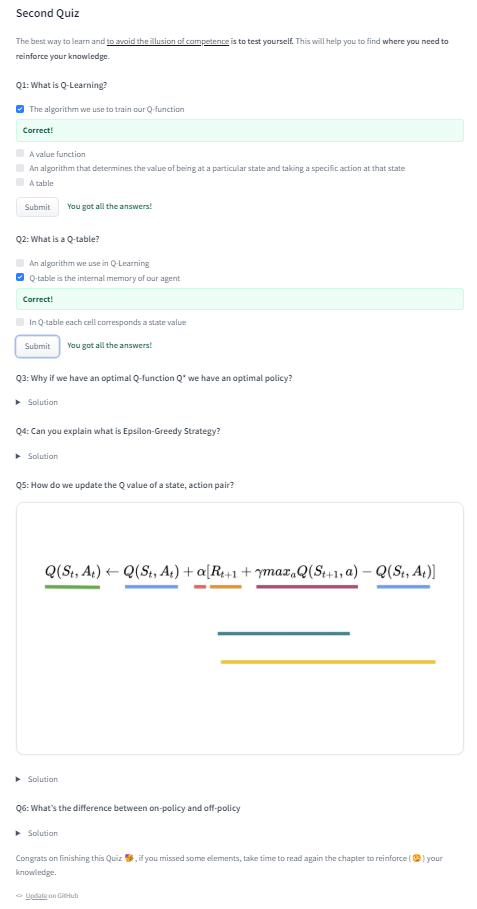
\includegraphics[width=0.8\textwidth]{../Img/Huggingface_DRL/unit2_quiz.png}
\end{figure}
\begin{figure}[H]
    \centering
    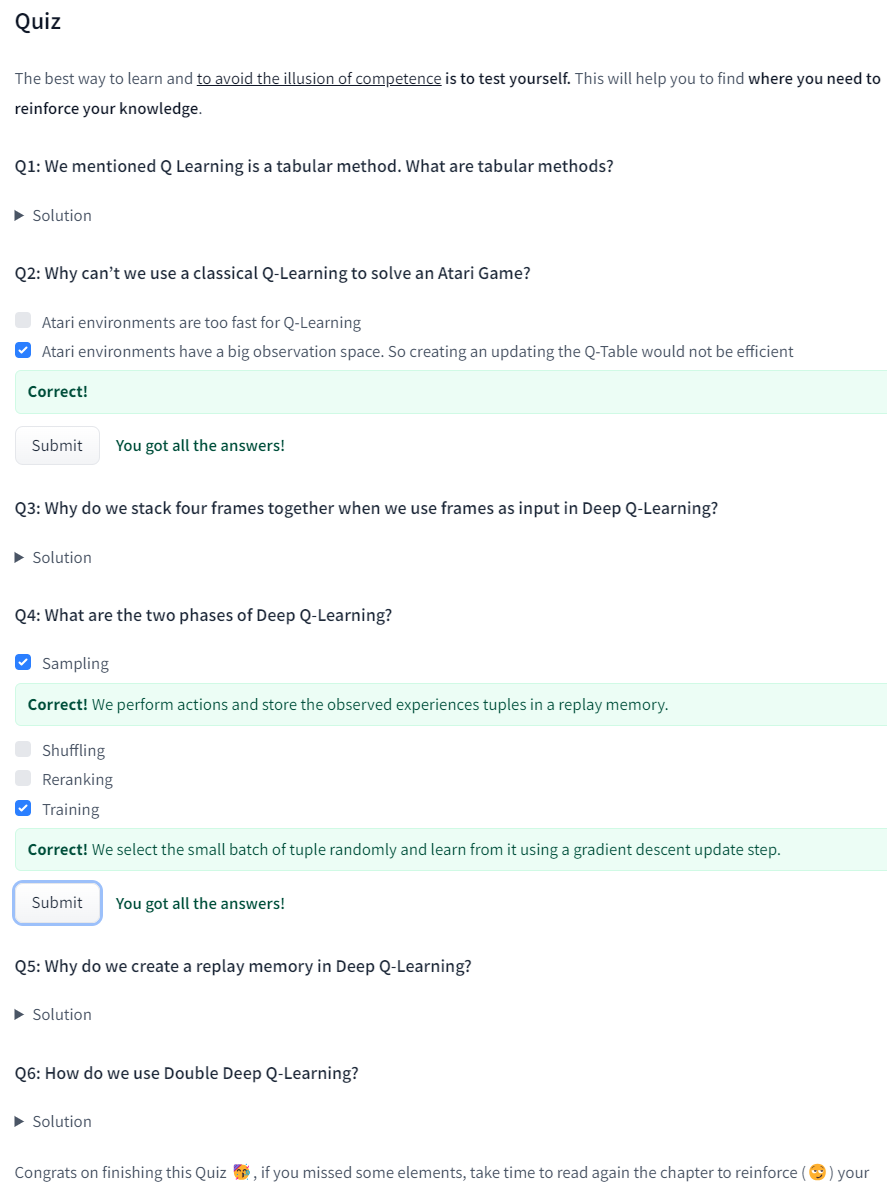
\includegraphics[width=0.8\textwidth]{../Img/Huggingface_DRL/unit3_quiz.png}
\end{figure}
\begin{figure}[H]
    \centering
    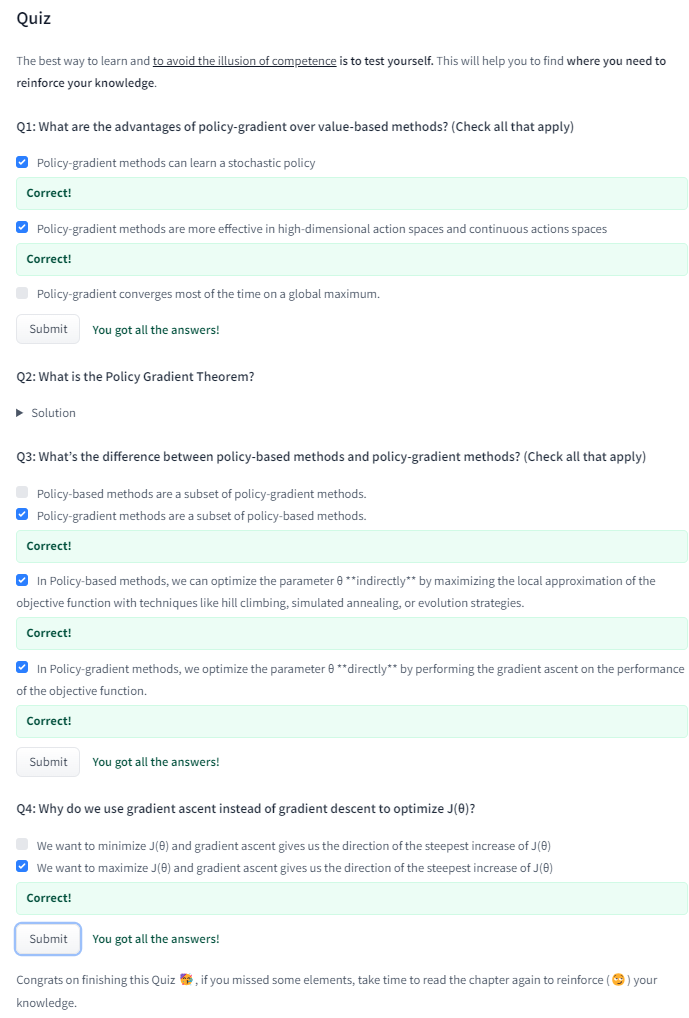
\includegraphics[width=0.8\textwidth]{../Img/Huggingface_DRL/unit4_quiz.png}
\end{figure}
\begin{figure}[H]
    \centering
    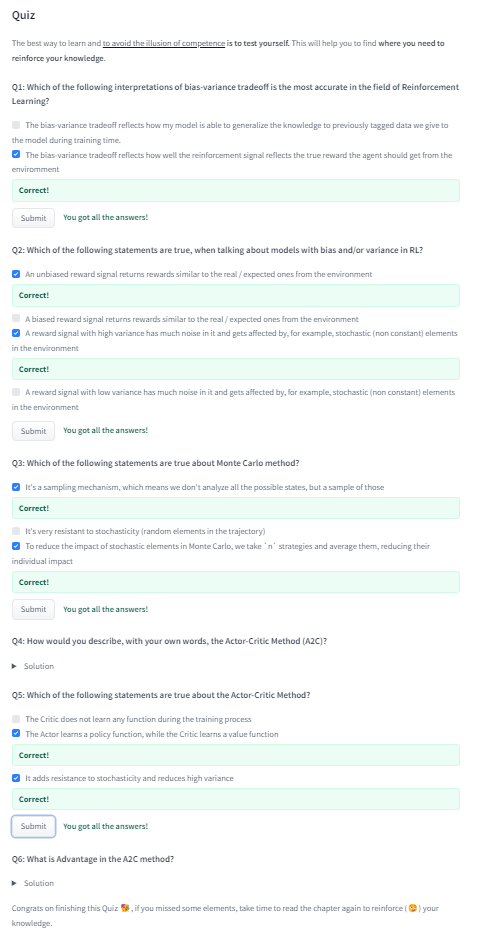
\includegraphics[width=0.8\textwidth]{../Img/Huggingface_DRL/unit6_quiz.png}
\end{figure}

\end{homeworkProblem}

\newpage